% Intro

%Several factors influence the execution plan of campaign on high performance computing resources (HPC), including resource capabilities, and resource dynamicity.
%Resource capabilities refer to the type and amount of computational resources, including: 
%\begin{inparaenum}[1)]
%\item computing capacity in terms of number of CPU cores, and possible accelerators, such as GPUs,
%\item main memory size, and
%\item filesystem in terms of size, and whether it is shared or not.
%\end{inparaenum}
%A resource is considered static when its availability remains constant over time, and dynamic when its availability changes.
%The user has, based on resource capacity and resource dynamicity, to evaluate how such capacity satisfies the campaign execution over the allocation period.
%These are complex and time consuming evaluations that depend on many variables, including resource usage policies, and amount of resources consumed by the campaign’s workflows.

%Scientific workflows are mainly executed by utilizing dedicated workflow management frameworks (WMF), such as RADICAL-Ensemble Toolkit~\cite{balasubramanian2018harnessing}, Pegasus~\cite{deelman2015pegasus} and others.
%These frameworks offer runtime capabilities, such as task execution, data dependency resolution, and workflow definition and monitoring.
%Given a set of resources and a walltime, WMF try to maximize resource utilization and minimize time to completion.
%WMF assume that the user selects sufficient resources and walltime to execute the workflow.
%Some workflow management frameworks, such as Dask~\cite{rocklin2015dask} and Airflow~\cite{airflow}, provide capabilities to elastically adapt resources, by scaling up or down, based on the current state of execution.
%In addition, some  WMFs~\cite{deelman2015pegasus} may support the concurrent execution of multiple workflows as independent entities, but not a single unified entity to achieve a single objective.
%Providing a campaign manager with capabilities to plan, monitor, and adapt the execution of a campaign becomes therefore desirable.
%Such a system can utilize campaign makespan calculations, alongside workflow execution capabilities, to automate campaign planning and execution. 

%Calculating the makespan of a computational campaign depends on workflow characteristics, workflow dependencies, campaign dynamicity, and resource dynamicity.
%Task execution time depends on parallelism, coordination between tasks, task characteristics~\cite{khoshlessan2017parallel}, the framework used to support task execution~\cite{paraskevakos2018task}, and resource dynamicity and performance variations~\cite{paraskevakos2019workflow, pouchard2019computational}.

%Based on workflow tasks’ characteristics, resources may need to be configured with different execution engines.
%Compute intensive applications on HPC resources are mainly executed via OpenMP/MPI benefiting from parallelism at scale, while data intensive application are parallelized  via data parallel frameworks such as Spark~\cite{zaharia2010spark}, or Dask~\cite{rocklin2015dask}.
%Traditionally, HPC resources are designed to optimize the execution of MPI tasks, leaving data-parallel frameworks largely unsupported.
%In Ref.~\cite{luckow2016hadoop}, we show how a pilot-based middleware~\cite{merzky2019using} can support the efficient and scalable execution of data-parallel applications on HPC resources.
%Such capabilities are necessary to support and plan the execution of a data-intensive campaign.



% Proposed topic

%Campaigns from the biomolecular and earth sciences are diverse in terms of composition, number and size of workflow members, and dynamicity. \mtnote{What does ``composition'' stand for in this context?}
%Biomolecular science campaigns may be comprised of a small number of workflows with millions of tasks, or thousands of workflows with tens to hundreds tasks~\cite{dakka2018high}. \mtnote{And everything in between these two boundaries?}
%Earth sciences campaigns, especially those which use VHR \mtnote{expand if not used before} satellite imagery, comprise of workflows with thousands of tasks.
%The number of workflows depends on the number of images the user has access to as well as the time they are able to obtain imagery.
%These workflows can be static~\cite{paraskevakos2019workflow} or dynamic~\cite{dakka2018high}. \mtnote{Did we explained why campaigns from these two science domains are interesting for this proposal?}

% ------------------------------------------------------------------------------
% Scientific campaigns
%Several factors influence the execution plan of campaign on high performance computing resources (HPC), including resource capabilities, and resource dynamicity.
%Resource capabilities refer to the type and amount of computational resources, including: 
%\begin{inparaenum}[1)]
%\item computing capacity in terms of number of CPU cores, and possible accelerators, such as GPUs,
%\item main memory size, and
%\item filesystem in terms of size, and whether it is shared or not.
%\end{inparaenum}
%A resource is considered static when its availability remains constant over time, and dynamic when its availability changes.
%The user has, based on resource capacity and resource dynamicity, to evaluate how such capacity satisfies the campaign execution over the allocation period.
%These are complex and time consuming evaluations that depend on many variables, including resource usage policies, and amount of resources consumed by the campaign’s workflows.

%Scientific workflows are mainly executed by utilizing dedicated workflow management frameworks (WMF), such as RADICAL-Ensemble Toolkit~\cite{balasubramanian2018harnessing}, Pegasus~\cite{deelman2015pegasus} and others.
%These frameworks offer runtime capabilities, such as task execution, data dependency resolution, and workflow definition and monitoring.
%Given a set of resources and a walltime, WMF try to maximize resource utilization and minimize time to completion.
%WMF assume that the user selects sufficient resources and walltime to execute the workflow.
%Some workflow management frameworks, such as Dask~\cite{rocklin2015dask} and Airflow~\cite{airflow}, provide capabilities to elastically adapt resources, by scaling up or down, based on the current state of execution.
%In addition, some  WMFs~\cite{deelman2015pegasus} may support the concurrent execution of multiple workflows as independent entities, but not a single unified entity to achieve a single objective.
%Providing a campaign manager with capabilities to plan, monitor, and adapt the execution of a campaign becomes therefore desirable.
%Such a system can utilize campaign makespan calculations, alongside workflow execution capabilities, to automate campaign planning and execution. 
%Calculating the makespan of a computational campaign depends on workflow characteristics, workflow dependencies, campaign dynamicity, and resource dynamicity.
%Task execution time depends on parallelism, coordination between tasks, task characteristics~\cite{khoshlessan2017parallel}, the framework used to support task execution~\cite{paraskevakos2018task}, and resource dynamicity and performance variations~\cite{paraskevakos2019workflow, pouchard2019computational}.

%Based on workflow tasks’ characteristics, resources may need to be configured with different execution engines.
%Compute intensive applications on HPC resources are mainly executed via OpenMP/MPI benefiting from parallelism at scale, while data intensive application are parallelized  via data parallel frameworks such as Spark~\cite{zaharia2010spark}, or Dask~\cite{rocklin2015dask}.
%Traditionally, HPC resources are designed to optimize the execution of MPI tasks, leaving data-parallel frameworks largely unsupported.
%In Ref.~\cite{luckow2016hadoop}, we show how a pilot-based middleware~\cite{merzky2019using} can support the efficient and scalable execution of data-parallel applications on HPC resources.
%Such capabilities are necessary to support and plan the execution of a data-intensive campaign.

%As a result, calculating the makespan of the campaign for based on workflow grouping, execution order, and workflow to resource mapping becomes important.
%The combination of workflow grouping, execution order, and workflow to resource mapping that produces a makespan which satisfies the computational objective of the campaign defines the execution plan of the campaign.

%Scientific workflows are generally described by direct acyclic graphs (DAG), where the nodes are tasks and the edges are dependencies.
%A subset of this general description of workflows are those which can be represented via the Pipeline, Stage, Task (PST) model~\cite{balasubramanian2018harnessing}. \mtnote{As discussed, EnTK and PST are implementation details.}
%The PST model describes workflows as a set of pipelines, where each pipeline is a sequence of stages.
%Each stage then is a set of tasks that need to be executed.
%Concurrency is achieved at the level of pipelines and the level of tasks. 
%Based on our use cases, we are particularly interested in scientific campaigns comprised by workflows that can be described via the PST model. \mtnote{Why?}
%Figure~\ref{fig:bio_earth_workflows} shows two example workflows from the biomolecular sciences (Fig.~\ref{fig:bio_workflow}) and the earth sciences (Fig.~\ref{fig:earth_workflow}). 

%\begin{figure*}[ht!]
%    \centering
%    \begin{subfigure}[b]{0.45\textwidth}
%         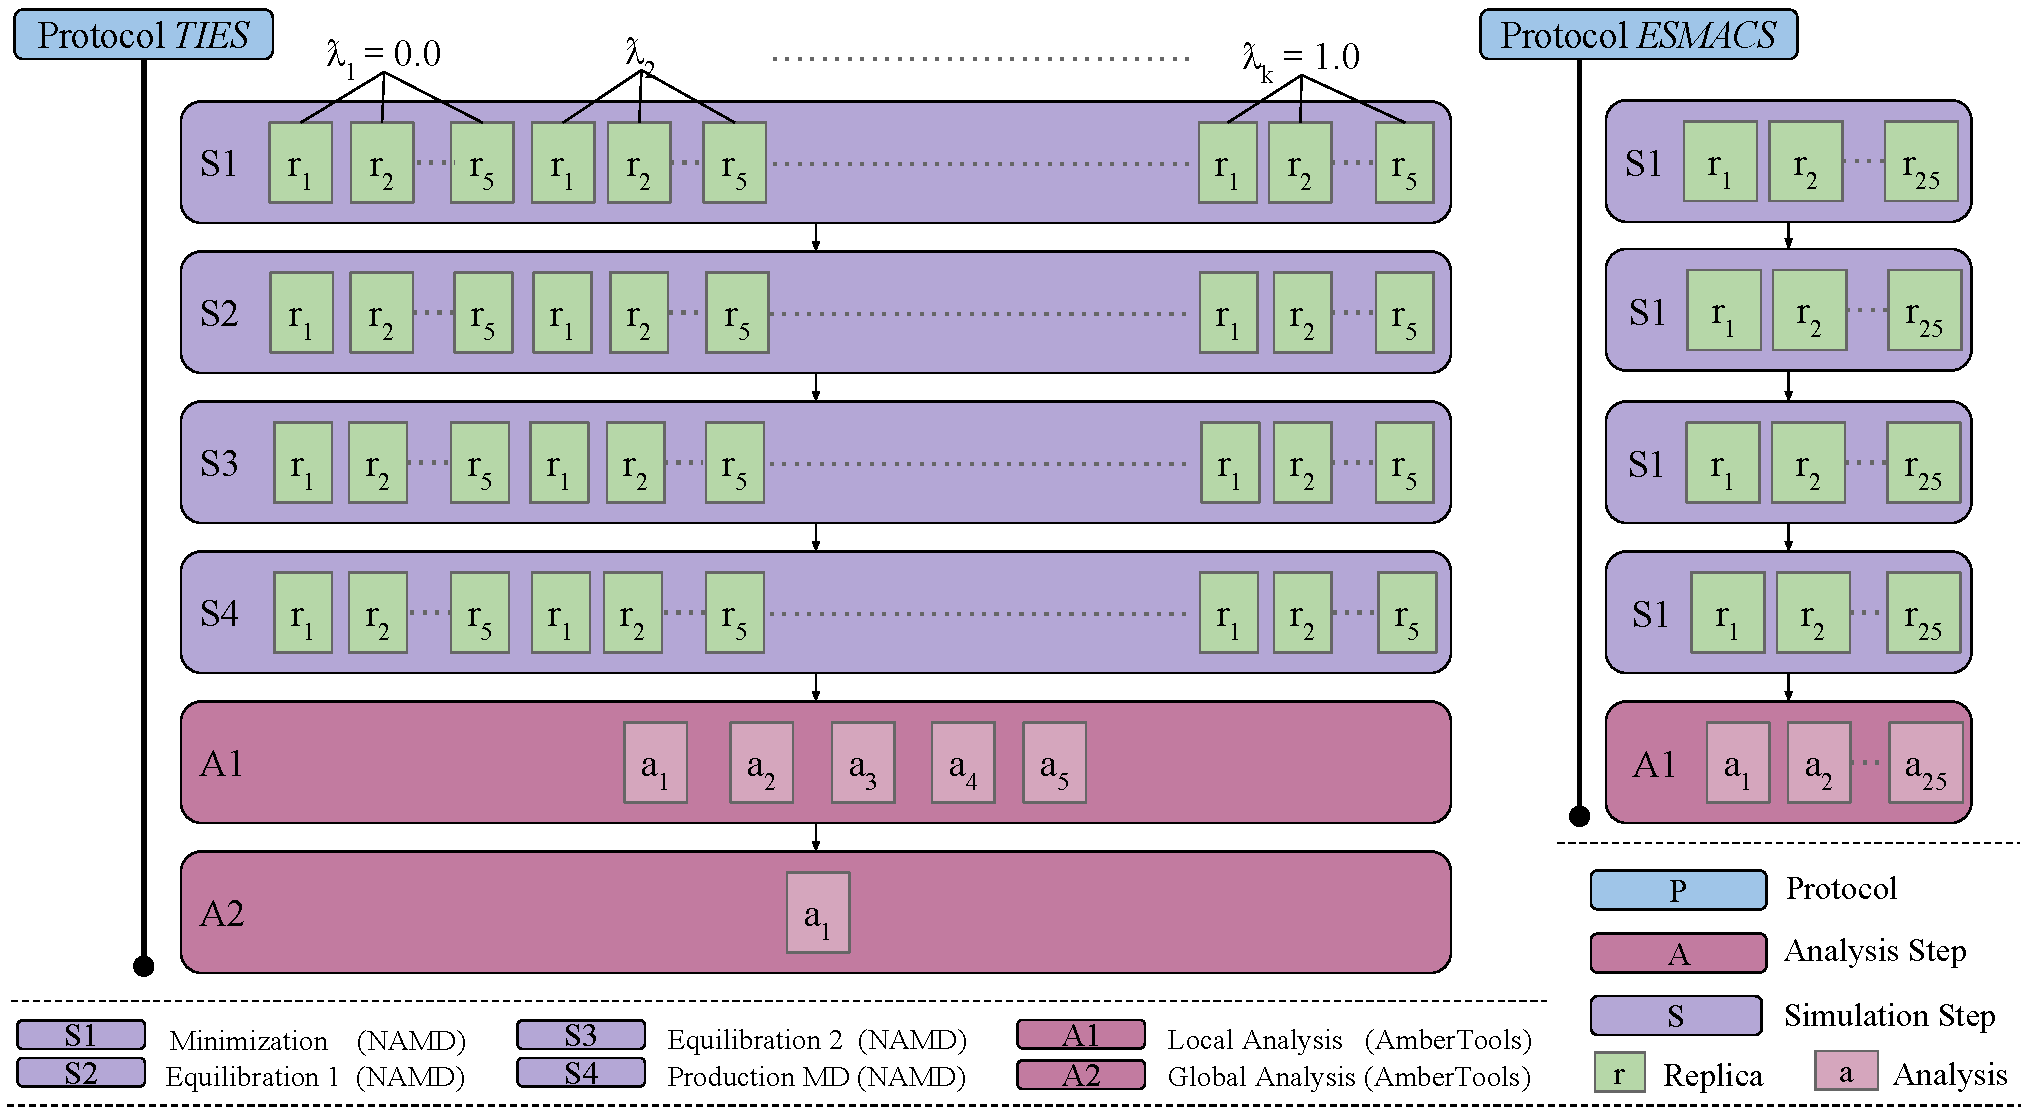
\includegraphics[width=\linewidth]{figures/bio_workflow.pdf}
%        \caption{}
%        \label{fig:bio_workflow}
%    \end{subfigure}%
%    ~ 
%    \begin{subfigure}[b]{0.45\textwidth}
%        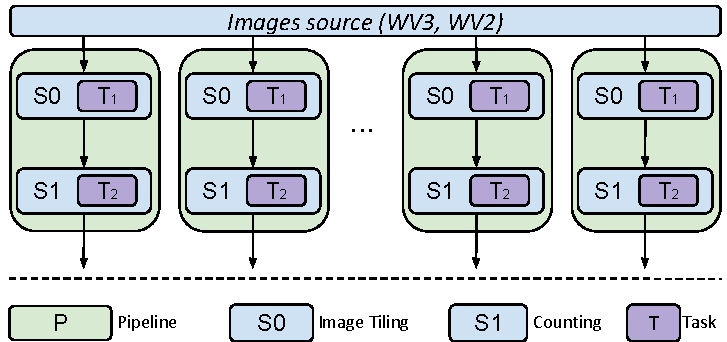
\includegraphics[width=\linewidth]{figures/earth_workflow.pdf}
%        \caption{}
%        \label{fig:earth_workflow}
%    \end{subfigure}
%    \caption{Biomolecular and Earth Science example workflows. \ref{fig:bio_workflow} Biomolecular workflow based on PST model example~\cite{dakka2018concurrent}; \ref{fig:earth_workflow} Earth science workflow based on PST model example~\cite{paraskevakos2019workflow}}\label{fig:bio_earth_workflows}
%\end{figure*}

%Computational campaigns resource requirements can be heterogeneous and cover a broad spectrum of resource types and numbers.
%Biomolecular science software tools support MPI/OpenMP, GPUs, and other accelerators, such as Intel Phi processors~\cite{cheatham2015impact} for executing either physical systems simulations or trajectory data analysis. \mtnote{simulations of? Analysis of?}
%In addition, some biomolecular analysis tool require specific computational environment or frameworks, such as Parallel MDAnalysis~\cite{fan2019pmda}, HiMach~\cite{tiankai2008scalable}.\mtnote{expand acronym, add other examples.}.
%Earth sciences applications, based on imagery, use workflows that execute a series of CPU based preprocessing, and eventually execute a computer vision algorithm on GPUs~\cite{paraskevakos2019workflow}\mtnote{This is specific to the applications you worked on, not necessarily true for all workflows used by the earth sciences communities. This comment seems to apply also to all the other examples of this paragraph}.


%The makespan of a campaign can be \mtnote{missing verb: derived maybe?} from a simple arithmetics calculation to a complex problem, depending on the heterogeneity of the campaign's workflows, maximum concurrency and resource dynamicity. \mtnote{This seems to assume that the reader has to understand the relation between makespan, heterogeneity and dynamicity on her own. I would refine and explain better.}
%Workflows can be heterogeneous in space, i.e., the number of tasks and resource requirements, and in time, i.e., the execution time needed to execute.
%When workflows are the same in space and time, they are considered homogeneous.
%Assuming enough resources to execute a workflow, when a campaign consists of homogeneous workflows any order of workflow execution would provide the same makespan. 
%When heterogeneity is introduced, randomly ordering the workflows' execution provides different makespan for different instances of the ordering.
%This is especially true, when there are not enough resources to execute all the workflows concurrently.
%As a result, calculating the makespan of the campaign based on workflow order execution becomes important to decide whether the selected mapping satisfies or not the campaign's computational campaign \mtnote{``campaign's computational campaign'' makes no sense.}.


%There are several alternative methods and algorithms to calculate and optimize the makespan of a workflow~\cite{lu2019review}, including queuing networks~\cite{yao2019throughput,bao2019performance}, domain specific languages~\cite{carothers2017durango,maheshwari2016workflow}, and machine learning~\cite{witt2019predictive,pumma2017runtime}.
%Queuing networks will be of limited use because they require from the user to provide a queuing network equivalent of the campaign.
%As a result, having the user provide a queuing network representation of the campaign adds an additional layer of complexity. \mtnote{These two sentences are unclear, please revise.}
%Domain specific languages would require too much engineering effort to convert a workflow representation based on domain specific assumptions, e.g., MPI style workflow, or specific languages representation, e.g., Swift, to a PST model representation \mtnote{This is unconvincing: we choose to use the PST model and then we say that it requires too much effort? Remember: the argumentation here has to be `scientific', not just based on 'I want to use EnTK so this would require too much time'.}.
%Machine Learning approaches would require model training, validation and testing to produce a model \mtnote{Why would this be a problem?}.
%In addition, since the execution is done on dynamic resources, the model should be retrained after every workflow execution.


% ----------------------------------------------------------------------------
% Initial Assumptions
%We propose to extend HEFT to support execution of a computational campaign on dynamic resources \mtnote{and heterogeneous?}.
%When executing a workflows HEFT assumes that any available resource can execute the workflow's tasks \mtnote{Why this statement is relevant?}.
%In addition, when executing a workflow on HPC resources, it can be assumed that all the resources will be available during the execution of the workflows \mtnote{Explain further, you seem to be assuming the reader understand a lot of implications of what you are writing. This is generally untrue has the reader has a very different background from yours and never thought to what you are writing here before.}.
%These two assumptions are not necessarily true when a computational campaign is executed.
%As campaign's workflows are heterogeneous, not all resources will satisfy the space requirements for all the workflows \mtnote{why?}.
%Introducing resource dynamicity requires HEFT to take into account resource availability to decide on which resources it will schedule workflows.
%In addition, it should update the schedule as resources become unavailable.

%The Executor sub-component is responsible to execute and monitor the plan \mtnote{where is the plan coming from?} by interfacing with a WMF.
%Based on the plan the Makespan calculator decided, the Executor submits workflows to a WMF to execute on the selected resource.
%This requires the Executor to work upon multiple workflows concurrently \mtnote{and why is this important?}.
%In addition, it should monitor workflow execution and resource availability \mtnote{why?}.
%An important requirement for the executor is to identify the reason of a failing workflow.
%When the failure is because the resource is not available, the specific workflow may need to be rescheduled and the plan to be updated.

%As a result, the campaign manager will see a set of resources where workflows should be executed upon \mtnote{not sure  understand how this follows from your explanation of pilots.}.\textbf{}